\documentclass[aspectratio=169,dvipdfmx,hyperref={bookmarks=true}]{beamer}
\usepackage{graphicx}
\usepackage{url}
\usepackage{bm}
\usepackage[absolute,overlay]{textpos}
\newcommand{\thickhrulefill}{\leavevmode\leaders\hrule depth-1.2pt height 3.2pt\hfill\kern0pt}
\newcommand{\indicatewidth}[1]{\thickhrulefill{#1}\thickhrulefill}
 \usetheme{Boadilla}
 \setbeamertemplate{navigation symbols}{}
 \setbeamertemplate{footline}[page number]
 \usepackage{algorithmic}
\usepackage{algorithm}
\usepackage{capt-of}
%\usepackage[dvipdfmx]{hyperref} % \movieref を使う場合に必要
\usepackage[dvipdfmx]{movie15_dvipdfmx}
%\usepackage[dvipdfmx]{movie15}
\renewcommand{\kanjifamilydefault}{\gtdefault}% 既定をゴシック体に

 %\usepackage[colorgrid,gridunit=pt,texcoord]{eso-pic}
 \title{煙シミュレーションのための部分空間法の高速化}
 \author{須之内 俊樹}
 \institute{中央大学理工学研究科 情報工学専攻 \\形状情報処理研究室 23N8100018B}
 \date{2025年 2月 21日}
 \usepackage{pxjahyper}
 \begin{document}
 %%%%%%%%%%%%%%%%%%%%%%%%%%%%%%%%%%%%%%%%%%%%%%%%%%%%%%%%%%%%%%%%%
   \begin{frame}
 \maketitle
 \end{frame} 
 %%%%%%%%%%%%%%%%%%%%%%%%%%%%%%%%%%%%%%%%%%%%%%%%%%%%%%%%%%%%%%%%%
% \begin{frame}
 %\tableofcontents
% \frametitle{目次}
 %\end{frame}
  %%%%%%%%%%%%%%%%%%%%%%%%%%%%%%%%%%%%%%%%%%%%%%%%%%%%%%%%%%%%%%%%%
     \section{概要}
 \begin{frame}
 \frametitle{概要}
  \begin{block}{}
  \begin{itemize}
	%\item 流体と接する製品の設計・製造,流体の映像の生成などに利用.
	\item 流体と接する製品の設計・製造
	\item 物理的に正確なシミュレーション
\end{itemize}
\end{block}

 \end{frame}
%%%%%%%%%%%%%%%%%%%%%%%%%%%%%%%%%%%%%%%%%%%%%%%%%%%%%%%%%%%%%%%%%
   \section{研究背景}
 \begin{frame}
 \frametitle{研究背景}
   \framesubtitle{流体シミュレーション}
 \subsection{流体シミュレーション}
  \begin{block}{工業分野}
  \begin{itemize}
	\item 流体と接する製品の設計・製造
	\item 物理的に正確なシミュレーションが重要視
\end{itemize}
\end{block}
\begin{block}{CG分野}
\begin{itemize}
	\item 流体の映像の生成に利用.
	\item 計算負荷を少なくすること,流体の挙動が制御しやすいことが重要視.
	\item 物理的な正確さよりも,それらしさを重要視.
\end{itemize}
\end{block}

 \begin{block}{流体シミュレーションの課題}
  \begin{itemize}
\item 希薄な流体や,水飛沫は手法によっては再現できない.
\item 近年は高品質な映像が求められ,計算負荷が大きい.
%\item 部分空間法による計算負荷の削減に取り組む.
\end{itemize}
\end{block}
 \end{frame}
%%%%%%%%%%%%%%%%%%%%%%%%%%%%%%%%%%%%%%%%%%%%%%%%%%%%%%%%%%%%%%%%%
  \begin{frame}
  \frametitle{研究背景}
  \framesubtitle{流体シミュレーションの数理モデル}
    \begin{block}{ナビエ・ストークス方程式}
\[
\frac{\partial}{\partial t}\bm{u} = - (\bm{u} \boldsymbol{\cdot}\nabla) \bm{u} - \frac{1}{\rho}\nabla p + \nu\nabla^2\bm{u} + \bm{f}
\]
\[
\nabla\boldsymbol{\cdot}\bm{u} = 0
\]
\begin{itemize}
	\item $\bm{u}$,$\bm{f}$:位置$\bm{x}$での流体の速度,外力
	\item $p$,$\rho$,$\nu$:位置$\bm{x}$での流体の圧力,密度,粘性
	\item $\nabla = ( \frac{\partial}{\partial x}, \frac{\partial}{\partial y}, \frac{\partial}{\partial z})$
\end{itemize}
\end{block}
\end{frame}
%%%%%%%%%%%%%%%%%%%%%%%%%%%%%%%%%%%%%%%%%%%%%%%%%%%%%%%%%%%%%%%%%
  \begin{frame}
  \frametitle{研究背景}
  \framesubtitle{流体シミュレーションの数理モデル}
    \begin{block}{部分段階法}
\[
\frac{\partial}{\partial t}\bm{u} = - (\bm{u} \boldsymbol{\cdot}\nabla) \bm{u} - \frac{1}{\rho}\nabla p + \nu\nabla^2\bm{u} + \bm{f}
\]

\[
\frac{\partial}{\partial t}\bm{u} = - (\bm{u} \boldsymbol{\cdot}\nabla) \bm{u} - \frac{1}{\rho}\nabla p + \nu\nabla^2\bm{u} + \bm{f}
\]
\end{block}
\end{frame}
%%%%%%%%%%%%%%%%%%%%%%%%%%%%%%%%%%%%%%%%%%%%%%%%%%%%%%%%%%%%%%%%%
  \begin{frame}
  \frametitle{研究背景}
  \framesubtitle{流体シミュレーションの数理モデル}
    \begin{block}{部分段階法}
\[
\frac{\partial}{\partial t}\bm{u} = - (\bm{u} \boldsymbol{\cdot}\nabla) \bm{u} - \frac{1}{\rho}\nabla p + \nu\nabla^2\bm{u} + \bm{f}
\]

この式を,中間子$\bm{u}_0$から$\bm{u}_3$を用いて,以下のように各項ごとに分割して計算する.
\begin{equation}\label{eq:force}
	\bm{u}_0 =  \bm{u} (t)  - \varDelta t \bm{f} 
\end{equation} 
\begin{equation}\label{eq:advect}
	\bm{u}_1 (\bm{x}) = \bm{u}_0 (\bm{x}) - \varDelta t (\bm{u}_0(\bm{x})  \boldsymbol{\cdot}\nabla) \bm{u}_0(\bm{x})
	%\bm{u}_1(\bm{x}) = \bm{u}_0(\bm{x}  - \varDelta t \bm{u}_0)
\end{equation}
\begin{equation}\label{eq:diffusion}
	\bm{u}_2   =  \bm{u}_1 - \varDelta t \nu\nabla^2\bm{u}_1
\end{equation}
\begin{equation}\label{eq:pressure}
	\bm{u} (t + \varDelta t)= \bm{u}_3  =  \bm{u}_2 - \varDelta t \frac{1}{\rho}\nabla \bm{p} 
\end{equation} 
\end{block}
\end{frame}
%%%%%%%%%%%%%%%%%%%%%%%%%%%%%%%%%%%%%%%%%%%%%%%%%%%%%%%%%%%%%%%%%
  \begin{frame}
  \frametitle{研究背景}
  \framesubtitle{流体シミュレーションの数理モデル}
    \begin{block}{部分段階法}
\[
\frac{\partial}{\partial t}\bm{u} = - (\bm{u} \boldsymbol{\cdot}\nabla) \bm{u} - \frac{1}{\rho}\nabla p + \nu\nabla^2\bm{u} + \bm{f}
\]

\[
	\bm{u}_0 =  \bm{u} (t)  - \varDelta t \bm{f} 	
\]
\[
	\bm{u}_1(\bm{x}) = \bm{u}_0(\bm{x}  - \varDelta t \bm{u}_0)
\]
\[
	\bm{u}_2   =  \bm{V}\bm{u}_1
\]
\[
	\bm{b} = \bm{W}\bm{u}_2
\]
\[
	\bm{p} = \bm{A}^{-1}\bm{b}
\]
\[
	\bm{u}_3  =  \bm{u}_2 - \bm{Y}\bm{p} 
\]
\end{block}
\end{frame}

%%%%%%%%%%%%%%%%%%%%%%%%%%%%%%%%%%%%%%%%%%%%%%%%%%%%%%%%%%%%%%%%%

\begin{frame}
 \frametitle{研究背景}
   \framesubtitle{先行研究}
\begin{columns}[T]
	\begin{column}{0.6\linewidth}
	\begin{block}{Visual Simulaton of Smoke \cite{fedkiw} [Fedkiw et al. 2001]}
		\begin{itemize}
		\item CGにおいて広く用いられる煙のオフラインシミュレーション手法.
		\item 密度を計算した後,ボリュームレンダリングを用いて描画.
		\item 陰解法による計算の安定性.
		\item 計算量は空間解像度に依存.
	\end{itemize}
	\end{block}
	
	\begin{block}{手法の課題}
		 近年の高品質な映像に不向き
	\end{block}
	%\begin{algorithm}[H]
    	%	\caption{Visual Simulation of Smoke}
       	 %\label{alg1}
        	%	\begin{algorithmic}[1]
         %               \STATE 重力,煙の浮力を計算し,速度を更新.
         %               \STATE semi-Lagragian法を用いて移流項を計算.
          %              \STATE コリンの射影法を用いて圧力項を計算.
           %             \STATE 密度,温度をsemi-Lagragian法を用いて更新.
              %          \STATE 密度の値を用いてレンダリング.
            %	\end{algorithmic}
	%\end{algorithm}
    	\end{column}
	\begin{column}{0.4\linewidth}
	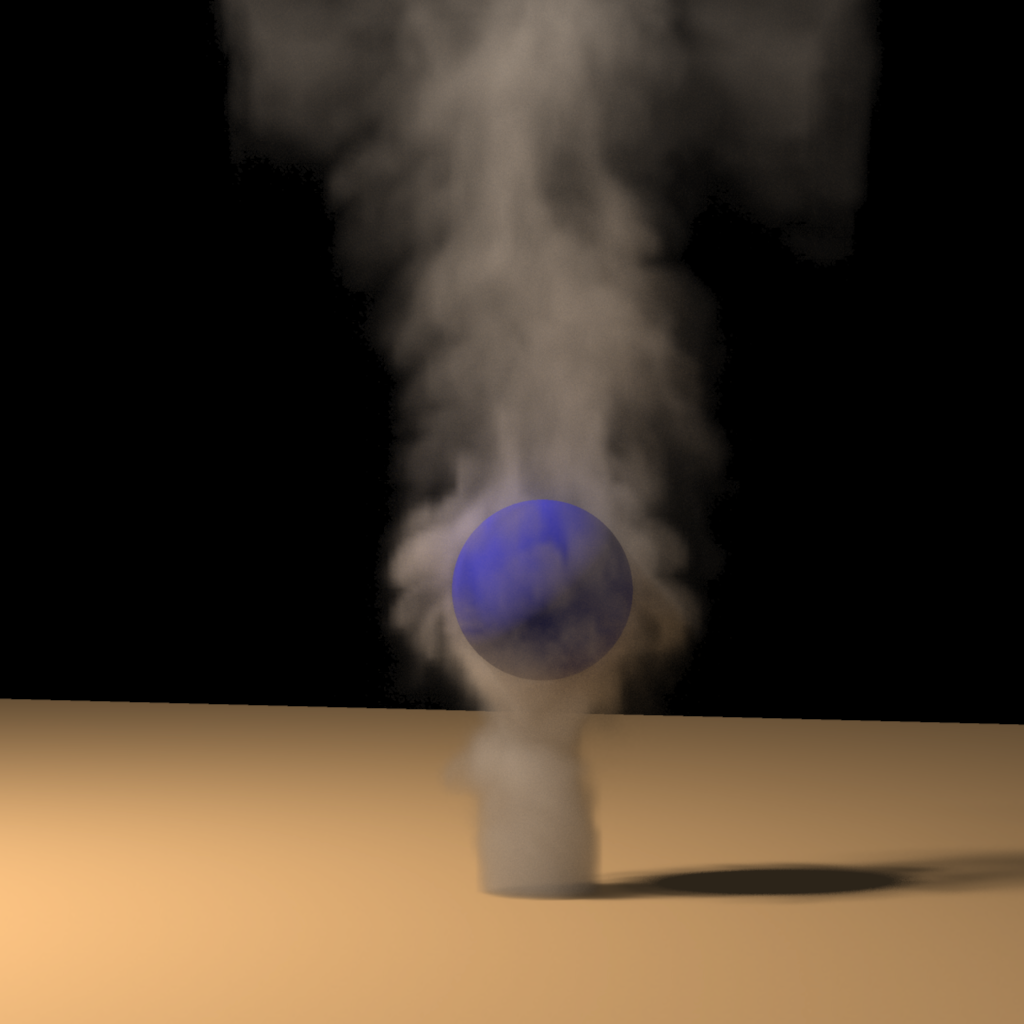
\includegraphics[width=0.8\linewidth]{images/vss-0017.png}
    	\end{column}
    \end{columns}
 \end{frame}
  %%%%%%%%%%%%%%%%%%%%%%%%%%%%%%%%%%%%%%%%%%%%%%%%%%%%%%%%%%%%%%%%%
\begin{frame}
 \frametitle{研究背景}
    \framesubtitle{先行研究}
   \begin{block}{ボリュームレンダリング}
   \begin{itemize}
 	\item 3次元空間の全てのボクセル値を可視化画像に反映させるレンダリング手法.
	\item 透明度を考慮したレンダリングに用いられる.
	\item サーフェスレンダリングは物体表面のみ可視化される.
\end{itemize}
\end{block}
\begin{columns}[T]
	\begin{column}{0.6\linewidth}
	\begin{algorithm}[H]
    		\caption{Axis Alined slice-based Volume Rendering}
       	 \label{alg1}
        		\begin{algorithmic}[1]
                        \STATE x,y,z軸の中から,視線方向に近いものを選ぶ.
                        \STATE 軸に垂直な平面(スライス)を,アルファブレンディングして描画.
                        \[{\rm{I_n}}(\bm{x})= \alpha_n(\bm{x})c_n(\bm{x}) + (1-\alpha_n(\bm{x})){\rm{I_{n-1}}}(\bm{x})\]
                        \[\alpha(\bm{x}) = 1 - exp(-\rho(\bm{x})\Delta s)\]
            	\end{algorithmic}
	\end{algorithm}
    	\end{column}
	
	\begin{column}{0.4\linewidth}
	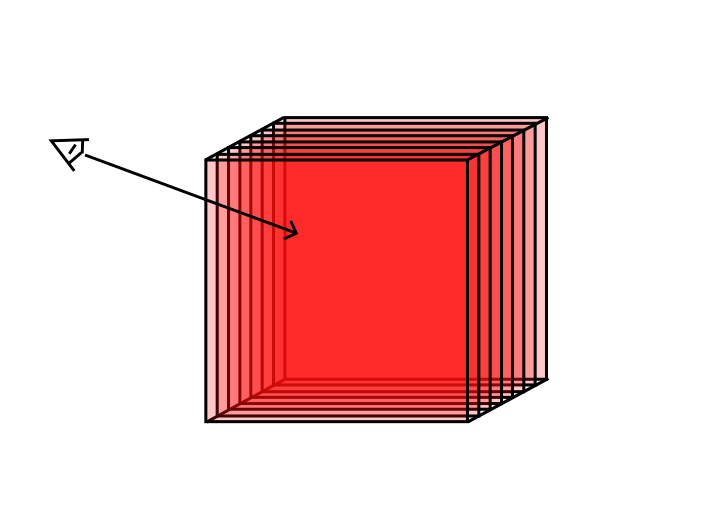
\includegraphics[width=\linewidth]{images/slice_base.png}
    	\end{column}
    \end{columns}
 \end{frame}

  %%%%%%%%%%%%%%%%%%%%%%%%%%%%%%%%%%%%%%%%%%%%%%%%%%%%%%%%%%%%%%%%%

   \begin{frame}
  \frametitle{部分空間法(subspace method)}
 \subsection{部分空間法}
\begin{block}{部分空間法\cite{subspace} [Kim et al. 2013]}
\begin{itemize}
\item 行列の低ランク近似を用いた手法.

 \item シミュレーションの前処理として,$n$次元ベクトル$\bm{x}$を$r$次元ベクトル$\bm{y}$に変換する$n \times r$行列$\mathbf{A}$を考える.
 \[
 \bm{y} = \mathbf{A}\bm{x}
 \]
 
	\item $\bm{y}$を用いてシミュレーションを行い,$\bm{x} = \mathbf{A}^{T}\bm{y}$を用いて$\bm{x}$を求める.
	\item 空間解像度を保ったまま高速化可能.
\end{itemize}
\end{block}
\centering
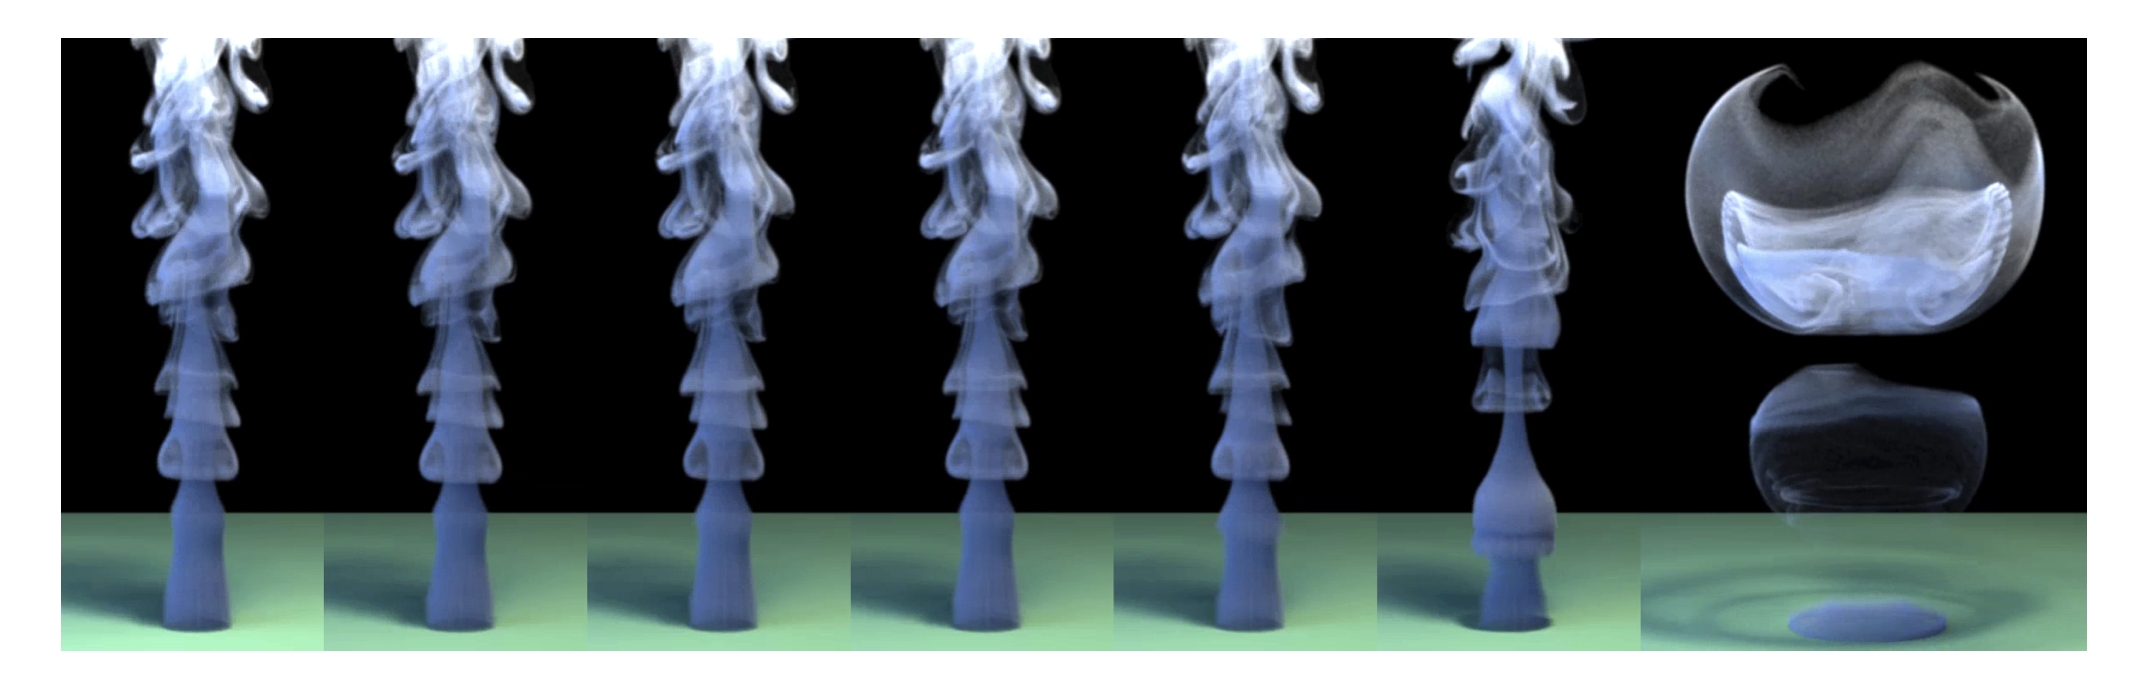
\includegraphics[width=0.7\linewidth]{images/subspace.png}
 \end{frame}
%%%%%%%%%%%%%%%%%%%%%%%%%%%%%%%%%%%%%%%%%%%%%%%%%%%%%%%%%%%%%%%%%
\begin{frame}
  \frametitle{部分空間法(subspace method)}
   \begin{block}{Snapshot固有直交分解}
   \begin{itemize}
   \item 既存のシミュレーションの時系列データを$m$個用いて,行列$\mathbf{A}$を作成する手法.
   
\item 空間解像度を$n$とする.一般に,$n \gg m \gg r$ 
\item 時刻$t$の速度ベクトル$\bm{u_t}$を用いて,$3n\times m$行列$\mathbf{U}$を定義する.

	 \[ \mathbf{U} = 
        		\begin{bmatrix}
   | & | &  & |\\
   \bm{u}_0 & \bm{u}_1 &\cdots  & \bm{u}_{m-1} \\
   | & | &  & |
\end{bmatrix}
\]
\item 行列$\mathbf{A}$について,以下のエネルギーを考える.
\[
min || \mathbf{U} -  \mathbf{A}\mathbf{A}^T \mathbf{U}||^2_F
\]

\item $\mathbf{A}$を$\mathbf{U}^T\mathbf{U}$の固有ベクトルとすることで最小化できる.
\item snapshotの数,削減後の次元の数が多いほど,削減前との誤差が少なくなる.
\end{itemize}
\end{block}

 \end{frame}
%%%%%%%%%%%%%%%%%%%%%%%%%%%%%%%%%%%%%%%%%%%%%%%%%%%%%%%%%%%%%%%%%
\begin{frame}
\frametitle{部分空間法の課題}
\subsection{部分空間法の課題}
	\begin{block}{空間計算量}
		一般に,
		\[64^3 \le n \le 1024^3\]
		\[30 \le r \le 150\]

   		\begin{itemize}
			\item $n = 256^3$,$r=50$のとき,行列$\mathbf{A}$のために10GBほど必要.
   			\item 削減後の次元の数に制限.
   			\item GPUによる高速化が不可能.
		\end{itemize}
	\end{block}

	\begin{block}{表現の限界}
 		\begin{itemize}
		\item 既存のシミュレーションと大幅に異なる表現.
		%\item 格子1つ分以下の領域の流れ.
	\end{itemize}
	\end{block}
\end{frame}
%%%%%%%%%%%%%%%%%%%%%%%%%%%%%%%%%%%%%%%%%%%%%%%%%%%%%%%%%%%%%%%%%
\section{改善手法}
\begin{frame}
\frametitle{改善手法}
\begin{block}{離散コサイン変換(DCT)を用いた行列の圧縮と展開\cite{subspaceDCT} [Jones et al. 2016] %\cite{Ishida}
}
	\begin{itemize}
		\item $8\times8\times8$個の格子を1ブロックとする.
		\item 1ブロックずつ展開し,GPUにデータを送信する.
	\end{itemize}
	\begin{itemize}
		\item 圧縮率が高すぎると視覚的に問題.
		%\item \cite{Ishida}ブロックの境界付近の計算の際,ブロック外のデータが必要.
		\item より疎な行列による空間計算量の削減が可能であるとされる.
	\end{itemize}
\end{block}

\begin{block}{領域分割\cite{tile}  [Wicke et al. 2009]}
	\begin{itemize}
		\item シミュレーション空間を分割し,小領域の計算を繰り返す.
		\item 速度の発散を0にするような分割を行う.
		%\item 既存のシミュレーション結果と異なる表現に対応.
		\item 計算誤差は大きく,計算負荷が増加する.
	\end{itemize}
	
\end{block}
領域分割後の小領域に,離散コサイン変換を適用.更なる空間計算量の削減.

計算結果の精度が低下する.
 \end{frame}

  %%%%%%%%%%%%%%%%%%%%%%%%%%%%%%%%%%%%%%%%%%%%%%%%%%%%%%%%%%%%%%%%%
 \begin{frame}
 \frametitle{実験}
流体と熱源を配置し,煙が立ち上る様子をシミュレーションした.

空間解像度 $n = 64^3$

シミュレーション 120ms/f,ボリュームレンダリング 15ms/f
\includemovie[autoplay, label=hikone]{80mm}{60mm}{movies/obstacle_origin.mp4}
\includemovie[autoplay, label=hikone]{80mm}{60mm}{movies/obstacle_dev1.mp4}
  \end{frame}
%%%%%%%%%%%%%%%%%%%%%%%%%%%%%%%%%%%%%%%%%%%%%%%%%%%%%%%%%%%%%%%%%
\begin{thebibliography}{99}
\beamertemplatetextbibitems

\bibitem{fedkiw}
R. Fedkiew, J. stam, H. Jensen. Visual simulation of smoke. In \textit{Proceedings of SIGGRAPH 01}, 15--22, 2001.

\bibitem{subspace}
T. Kim, J. Delaney. Subspace Fluid Re-Simulation. \textit{ACM Transactions on Graphics},32, (4): , 62:1--62:9, 2013.

\bibitem{subspaceDCT}
A. Jones, P. Sen, and T. Kim. Compressing fluid subspaces. \textit{Proceedings of the ACM SIGGRAPH/Eurographics Symposium on Computer Animation}, pp. 77--84, 2016.

\bibitem{tile}
M. Wicke, M. Stanton, and A. Treuille, Modular Bases for Fluid Dynamics. \textit{ACM Transactions on Graphics}, 39:1--39:8, 2009.

%\bibitem{Ishida}
%D. Ishida , R. Ando , S. Morishima. GPU smoke simulation on compressed DCT space.  \textit{Eurographics Short Papers}, pp. 5--8, 2019.

\end{thebibliography}
\end{document}